\documentclass[10pt]{article}
\usepackage[margin=2.3cm]{geometry}
\usepackage{graphicx,booktabs,xcolor,hyperref,enumitem,amssymb}
\hypersetup{colorlinks=true,linkcolor=blue!60!black,urlcolor=blue!60!black}
\setlist{nosep,leftmargin=1.4em}
\newcommand{\code}[1]{\texttt{\small #1}}
\title{\vspace{-1.4em}8B ASearcher arms: token-GRPO vs turn-PPO (75 steps, fast config)\\
\large Qwen3-8B-Base, ASearcher Base-35k unfiltered, 32-turn/16k, partial rollout\vspace{-0.5em}}
\author{Agentic-RL-CA rung-3 --- branch \code{sync-partial-rollout-poc}}
\date{2026-08-02}
\begin{document}\maketitle\vspace{-1.8em}

\section*{TL;DR}
Both arms completed 75 steps. \textbf{turn-PPO finishes ahead: val EM 0.561 vs GRPO's
0.520}, using \textbf{less than half the search volume} (6.5 vs 16.1 calls/question).
GRPO plateaued after step 50 while re-inflating turns (14.6$\to$17.0); turn-PPO kept
improving while holding $\sim$7.5 turns. Both roughly tripled the zero-shot baseline
(0.195). \textbf{This inverts the 4B filtered result} (GRPO 0.773 vs turn-PPO 0.496) ---
three confounds separate the settings (\S4). Single seed per arm; treat the 4-point gap at
step 50 and the 4.1-point final gap as suggestive, not decisive.

\section{Setup}
Identical for both arms except the estimator: Qwen3-8B-Base (RL from base), ASearcher
Base-35k \emph{unfiltered}, wiki-18/e5 top-5, 32-turn nominal horizon with 16k prompt +
clean context-overflow termination, 1024-token responses, full \code{<think>}+\code{<search>}
history, 256 prompts $\times$ group 5, lr 1e-6, 75 steps, val every 25 on a fixed
512-question set (greedy). Fast config: partial rollout (cycle 8, max\_age 4), dynamic
token-budget micro-batching, chunked prefill. GRPO uses KL-in-loss 1e-3; turn-PPO
(\code{gae\_turn}) uses no KL and a colocated critic with CPU offload.
Runs: \href{https://wandb.ai/rainyfields/ca-rung3-8b-asearcher}{\code{ca-rung3-8b-asearcher}}
(\code{*\_32turn\_fast75\_s0}).

\section{Results}
\begin{center}
\begin{tabular}{lrrrr}
\toprule
val step & 0 & 25 & 50 & \textbf{75}\\
\midrule
GRPO EM & 0.195 & 0.227 & 0.520 & \textbf{0.520}\\
GRPO turns & 8.17 & 17.14 & 14.62 & 17.04\\
GRPO searches & 7.56 & 16.73 & 13.68 & 16.08\\
\midrule
turn-PPO EM & 0.195 & 0.234 & 0.479 & \textbf{0.561}\\
turn-PPO turns & 8.17 & 11.02 & 7.88 & 7.49\\
turn-PPO searches & 7.56 & 10.58 & 6.96 & 6.49\\
\bottomrule
\end{tabular}
\end{center}

\begin{center}
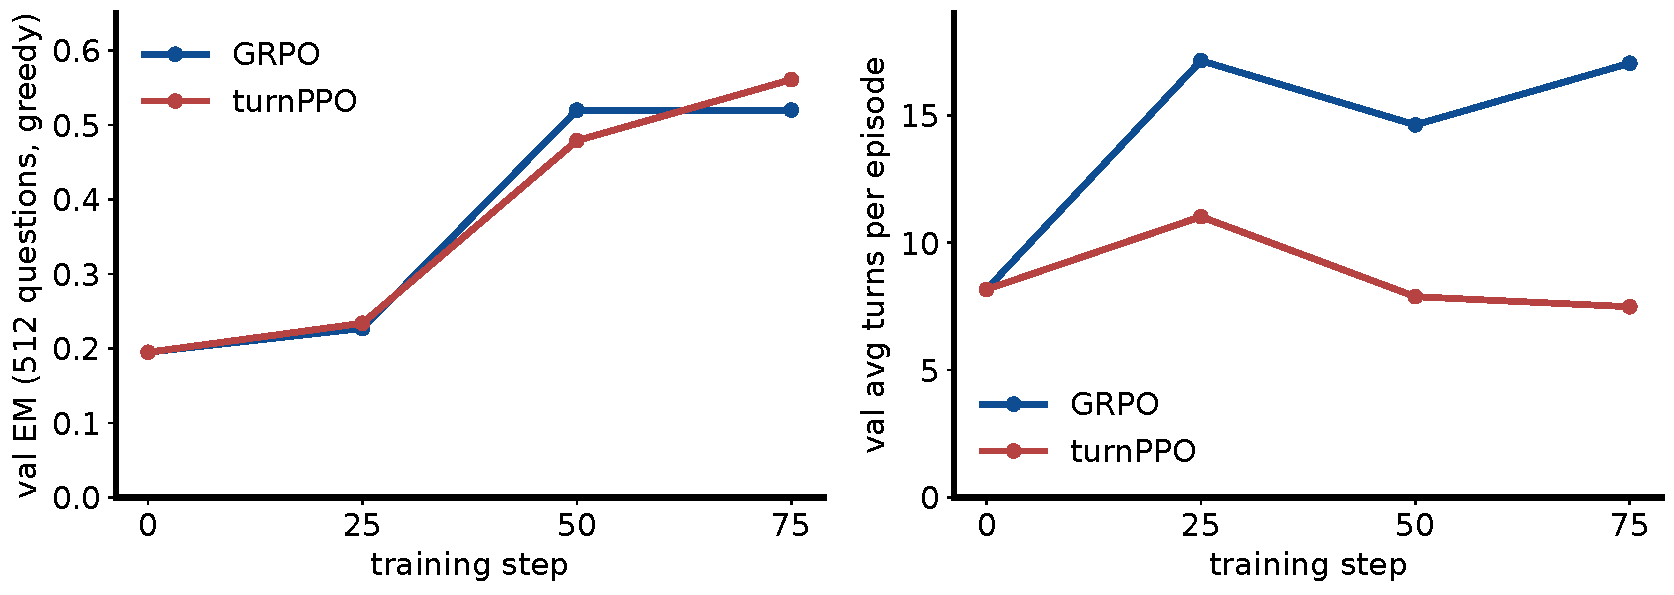
\includegraphics[width=0.98\linewidth]{assets/fig_arms_curves}\\[0.4em]
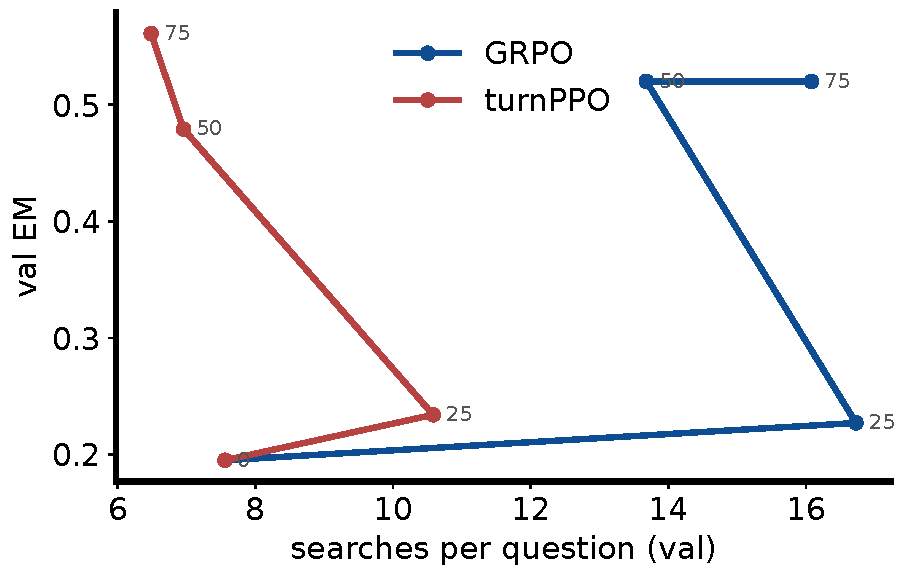
\includegraphics[width=0.56\linewidth]{assets/fig_em_vs_search}
\end{center}

\section{Reading the behaviour}
\begin{itemize}
\item \textbf{Both arms inflate turns early, then diverge.} At step 25 both push turn counts
up (GRPO 17.1, turn-PPO 11.0) with little EM gain --- exploration, not yet competence. From
step 25 to 50 both gain $\sim$0.25 EM; turn-PPO does so while \emph{cutting} turns to 7.9,
GRPO while cutting only to 14.6, then returning to 17.0 by step 75.
\item \textbf{turn-PPO is the efficient searcher.} Its per-turn value estimates penalise
turns that do not improve the return, so useless search is pruned. GRPO's single episode
return, broadcast to every turn, gives no such signal --- extra turns are free.
\item \textbf{Response length diverges too}: at step 75 GRPO's mean per-turn response
collapsed to 54 tokens (entropy 0.049) vs turn-PPO's 145 (entropy 0.026) --- GRPO learned
many short turns, turn-PPO fewer richer ones. Train success is equal (0.507 vs 0.514 at
temp 1.0), so the val gap is a greedy-decode/efficiency effect, not a rollout-quality gap.
\item \textbf{Cost implication}: at equal EM, turn-PPO's trajectories are $\sim$2$\times$
cheaper to generate --- relevant for the long-horizon budget discussion, since generation
dominates step time in the fast config.
\end{itemize}

\section{Why this may invert the 4B result}
The 4B comparison (p3v2, filtered Base) gave GRPO 0.773 vs turn-PPO 0.496. Three
differences, any of which could drive the flip:
\begin{enumerate}
\item \textbf{Data}: 4B ran on closed-book-filtered questions (search mandatory); 8B ran
unfiltered, where $\sim$40\% of successful trajectories use \emph{zero} searches (parametric
recall). Part of the 8B EM is recall, and the estimators may exploit that differently.
\item \textbf{Horizon}: 8-turn/16k (4B) vs 32-turn nominal (8B). Turn-level credit
assignment should matter more as the horizon grows --- consistent with turn-PPO winning here.
\item \textbf{Scale}: 4B-Instruct vs 8B-Base.
\end{enumerate}
Disentangling these needs at minimum an 8B filtered run (isolates the data confound); an
8-turn 8B run would isolate the horizon.

\section{Caveats}
Single seed per arm; 512-question val (a 4-point difference is $\sim$1 SE). GRPO's run
absorbed an OOM restart at $\sim$cycle 35 --- resumed cleanly from the step-25 checkpoint
(post-resume val reproduced 0.227 exactly) but replayed $\sim$10 cycles with a smaller
dynamic-batch token budget (20{,}480 vs 24{,}576); packing changes forward grouping, not
gradients. Both arms stopped at 75 steps mid-ascent for turn-PPO (still +0.08 over the last
25 steps), so neither number is a converged ceiling.

\section{Suggested next steps}
1) Seed replication before any headline claim. 2) 8B \emph{filtered} arms to remove the
recall confound. 3) If the efficiency result holds, it is itself a finding for the
benchmark: turn-level credit assignment buys search efficiency at long horizon, which the
episode-level baseline does not. 4) Cheaper compute is available: B200 runs this stack
1.53$\times$ faster end-to-end (\code{docs/reports/2026-08-01\_b200\_turnppo\_experiment.md}).
\end{document}
